\documentclass{beamer}

\usepackage[utf8]{inputenc}
\usepackage[T2A]{fontenc}
\usepackage[russian,english]{babel}
%\usepackage{tikz}
%\usetikzlibrary{tikzmark}
%\usetikzlibrary{calc}

\usepackage[font=scriptsize]{caption}
\setlength{\abovecaptionskip}{5pt plus 0pt minus 2pt} % Chosen fairly arbitrarily

\usepackage[backend=biber]{biblatex}
\addbibresource{../bib/ms-thesis.bib}
%\newcommand{\tikzmark}[1]{\tikz[remember picture] \node[coordinate] (#1) {#1};}


\usepackage{array}
\usepackage{xcolor}

\usepackage{hyphenat} % for using \nohyphens
%\usepackage{multirow} %Used for tables with merged cells
%\usepackage{collcell} %pdflatex.exe hangs without this one

\usepackage{booktabs}% http://ctan.org/pkg/booktabs
\newcommand{\tabitem}{~~\llap{\textbullet}~~}


%\RequirePackage{aaltologo}
%\RequirePackage{beamercolorthemeAalto}
%\RequirePackage{beamerthemeAalto}

% There are many different themes available for Beamer. A comprehensive
% list with examples is given here:
% http://deic.uab.es/~iblanes/beamer_gallery/index_by_theme.html
% You can uncomment the themes below if you would like to use a different
% one:
%\usetheme[school={SCI}]{Aalto}
%\usetheme{AnnArbor}
%\usetheme{Antibes}
%\usetheme{Bergen}
%\usetheme{Berkeley}
%\usetheme{Berlin}
%\usetheme{Boadilla}
%\usetheme{boxes}
%\usetheme{CambridgeUS}
%\usetheme{Copenhagen}
%\usetheme{Darmstadt}
%\usetheme{default}
%\usetheme{Frankfurt}
%\usetheme{Goettingen}
%\usetheme{Hannover}
%\usetheme{Ilmenau}
%\usetheme{JuanLesPins}
%\usetheme{Luebeck}
%\usetheme{Madrid}
%\usetheme{Malmoe}
%\usetheme{Marburg}
\usetheme{Montpellier}
%\usetheme{PaloAlto}
%\usetheme{Pittsburgh}
%\usetheme{Rochester}
%\usetheme{Singapore}
%\usetheme{Szeged}
%\usetheme{Warsaw}


%\titlegraphic{\includegraphics[height=1cm,width=2cm]{logo1}}
%\titlegraphicii{\includegraphics[height=1cm,width=2cm]{logo2}}

\title{\nohyphens{\textbf{Automated~Analysis~of~Weak~Memory~Models}}}

% A subtitle is optional and this may be deleted
%\subtitle{Optional Subtitle}
\author{\textbf{Artem Yushkovskiy}\inst{1,2} \\ 
{\scriptsize MSc Candidate}
\\ \vspace{1em}
{\footnotesize\raggedleft Supervisors: \textbf{Assoc. Prof. Keijo Heljanko}\inst{1} \newline
\hphantom{Supervis} \textbf{Docent Igor I. Komarov}\inst{2} }
}%\small
%{\footnotesize%\raggedleft%does not work
%Supervisor 1: Assoc. Prof. Keijo Heljanko\inst{1} \newline
%Supervisor 2: Docent Igor I. Komarov\inst{2}
%}


\institute % (optional, but mostly needed)
{
  \inst{1}%
  Department of Computer Science, \\
  School of Science, \\
  \textbf{Aalto University} (Espoo, Finland)%
  \and
  \inst{2}%
  Faculty of Information Security \\
  and Computer Technologies, \\
  \textbf{ITMO University} (Saint Petersburg, Russia)%
}

\date{\scriptsize Espoo, Saint Petersburg, 2018}
% - Either use conference name or its abbreviation.
% - Not really informative to the audience, more for people (including
%   yourself) who are reading the slides online

%\subject{Computer Science}
% This is only inserted into the PDF information catalog. Can be left
% out. 

% If you have a file called "university-logo-filename.xxx", where xxx
% is a graphic format that can be processed by latex or pdflatex,
% resp., then you can add a logo as follows:

%\pgfdeclareimage[height=0.5cm]{university-logo}{}
%\logo{\pgfuseimage{university-logo}}

% Delete this, if you do not want the table of contents to pop up at
% the beginning of each subsection:
\AtBeginSubsection[]
{
  \begin{frame}<beamer>{Outline}
    \tableofcontents[currentsection,currentsubsection]
  \end{frame}
}

\usepackage{colortbl}
\definecolor{ltgrey}{rgb}{0.85,0.85,0.85}
\definecolor{dkblue}{rgb} {0,   0.1, 0.6}
\definecolor{dkred} {rgb} {0.6, 0.1, 0}
\renewcommand{\r}[1]{\ensuremath{\textcolor{dkred}{#1}}}
\renewcommand{\b}[1]{\ensuremath{\textcolor{dkblue}{#1}}}


% Let's get started
\begin{document}

\begin{frame}
  \titlepage
\end{frame}

\begin{frame}{Outline}
  \tableofcontents
  % You might wish to add the option [pausesections]
\end{frame}


\section{Introduction}

\subsection{Weak memory model-aware analysis}

\begin{frame}{Verification of concurrent software}
\framesubtitle{Example: Write-write reordering (by compiler)}
%1) mckenney  http://www.rdrop.com/users/paulmck/scalability/paper/whymb.2010.06.07c.pdf
%2) http://preshing.com/20120515/memory-reordering-caught-in-the-act/
\begin{table}
\centering
\ttfamily
\begin{tabular}{ |>{\color{dkblue}}l | >{\color{dkred}}l| }
\hline
\multicolumn{2}{|l|}{ \{ x=0; y=0; \}} \tabularnewline \hline
P & Q \\ \hline
$p_0$ : $x \leftarrow 1$   & $q_0$: $y \leftarrow 1$   \\
$p_1$ : $r_p \leftarrow y$ & $q_1$: $r_q \leftarrow x$ \\
\hline
\end{tabular}
\end{table}

%\tikzmark{p1} 
%\begin{tikzpicture}[remember picture, overlay]
%  \path[draw=red,thick,<->]<4-> (pic cs: p0) to [] (pic cs: p1);
%\end{tikzpicture}

\addtolength{\tabcolsep}{-3pt}

\def\firstrowcolor{}
\def\secondrowcolor{}
\hspace{-20pt}
\begin{minipage}{.25\textwidth}
\small
\onslide<2-> 
\begin{tabular}{ l r}
\rowcolor{ltgrey} $\b{p_0}, \b{p_1}, \r{q_0}, \r{q_1}$ & $(\b{0}; \r{1})$ \\
\rowcolor{ltgrey} $\r{q_0}, \r{q_1}, \b{p_0}, \b{p_1}$ & $(\b{1}; \r{0})$ \\
%\hline
\pause
\onslide<3-> 
$\b{p_0}, \r{q_0}, \b{p_1}, \r{q_1}$ & $(\b{1}; \r{1})$ \\
$\b{p_0}, \r{q_0}, \r{q_1}, \b{p_1}$ & $(\b{1}; \r{1})$ \\
$\r{q_0}, \b{p_0}, \b{p_1}, \r{q_1}$ & $(\b{1}; \r{1})$ \\
$\r{q_0}, \b{p_0}, \r{q_1}, \b{p_1}$ & $(\b{1}; \r{1})$ \\
%\hline
\pause
\end{tabular}
\end{minipage}
%
\hspace{5pt}
\begin{minipage}{.6\textwidth}
\small
\onslide<4->
%\vspace{-1em}
%"delay the effect of a store past any load from a different location."
\vspace{-11pt}
\begin{tabular}{ | l r | l r | l r }
\rowcolor{ltgrey} $\underline{\b{p_1}}, \underline{\b{p_0}}, \r{q_0}, \r{q_1}$ & $(\b{0}; \r{1})$  &  $\b{p_0}, \b{p_1}, \underline{\r{q_1}}, \underline{\r{q_0}}$ & $(\b{0}; \r{1})$  &  $\underline{\b{p_1}}, \underline{\b{p_0}}, \underline{\r{q_1}}, \underline{\r{q_0}}$ & $(\b{0}; \r{1})$ \\
\rowcolor{ltgrey} $\r{q_0}, \r{q_1}, \underline{\b{p_1}}, \underline{\b{p_0}}$ & $(\b{1}; \r{0})$  &  $\underline{\r{q_1}}, \underline{\r{q_0}}, \b{p_0}, \b{p_1}$ & $(\b{1}; \r{0})$  &  $\underline{\r{q_1}}, \underline{\r{q_0}}, \underline{\b{p_1}}, \underline{\b{p_0}}$ & $(\b{1}; \r{0})$ \\
$\underline{\b{p_1}}, \r{q_0}, \underline{\b{p_0}}, \r{q_1}$ & $(\b{0}; \r{1})$  &  $\b{p_0}, \underline{\r{q_1}}, \b{p_1}, \underline{\r{q_0}}$ & $(\b{0}; \r{1})$  &  $\underline{\b{p_1}}, \underline{\r{q_1}}, \underline{\b{p_0}}, \underline{\r{q_0}}$ & $(\b{0}; \r{0})$ \\
$\underline{\b{p_1}}, \r{q_0}, \r{q_1}, \underline{\b{p_0}}$ & $(\b{0}; \r{0})$  &  $\b{p_0}, \underline{\r{q_1}}, \underline{\r{q_0}}, \b{p_1}$ & $(\b{1}; \r{1})$  &  $\underline{\b{p_1}}, \underline{\r{q_1}}, \underline{\r{q_0}}, \underline{\b{p_0}}$ & $(\b{0}; \r{0})$ \\
$\r{q_0}, \underline{\b{p_1}}, \underline{\b{p_0}}, \r{q_1}$ & $(\b{1}; \r{1})$  &  $\underline{\r{q_1}}, \b{p_0}, \b{p_1}, \underline{\r{q_0}}$ & $(\b{0}; \r{0})$  &  $\underline{\r{q_1}}, \underline{\b{p_1}}, \underline{\b{p_0}}, \underline{\r{q_0}}$ & $(\b{0}; \r{0})$ \\
$\r{q_0}, \underline{\b{p_1}}, \r{q_1}, \underline{\b{p_0}}$ & $(\b{1}; \r{0})$  &  $\underline{\r{q_1}}, \b{p_0}, \underline{\r{q_0}}, \b{p_1}$ & $(\b{1}; \r{0})$  &  $\underline{\r{q_1}}, \underline{\b{p_1}}, \underline{\r{q_0}}, \underline{\b{p_0}}$ & $(\b{0}; \r{0})$ \\
\end{tabular}
\end{minipage}

\end{frame}



\begin{frame}{Verification of concurrent software}
\framesubtitle{Example: Store buffering (by hardware)}
\begin{center}
\scalebox{0.7}{
\ttfamily
\begin{tabular}{ |>{\color{dkblue}}l | >{\color{dkred}}l| }
\hline
\multicolumn{2}{|l|}{ \{ x=0; y=0; \}} \tabularnewline \hline
P & Q \\ \hline
$p_0$ : $x \leftarrow 1$   & $q_0$: $y \leftarrow 1$   \\
$p_1$ : $r_p \leftarrow y$ & $q_1$: $r_q \leftarrow x$ \\
\hline
\end{tabular}
}
\end{center}

\vspace{-5pt}
\begin{figure}
\centering
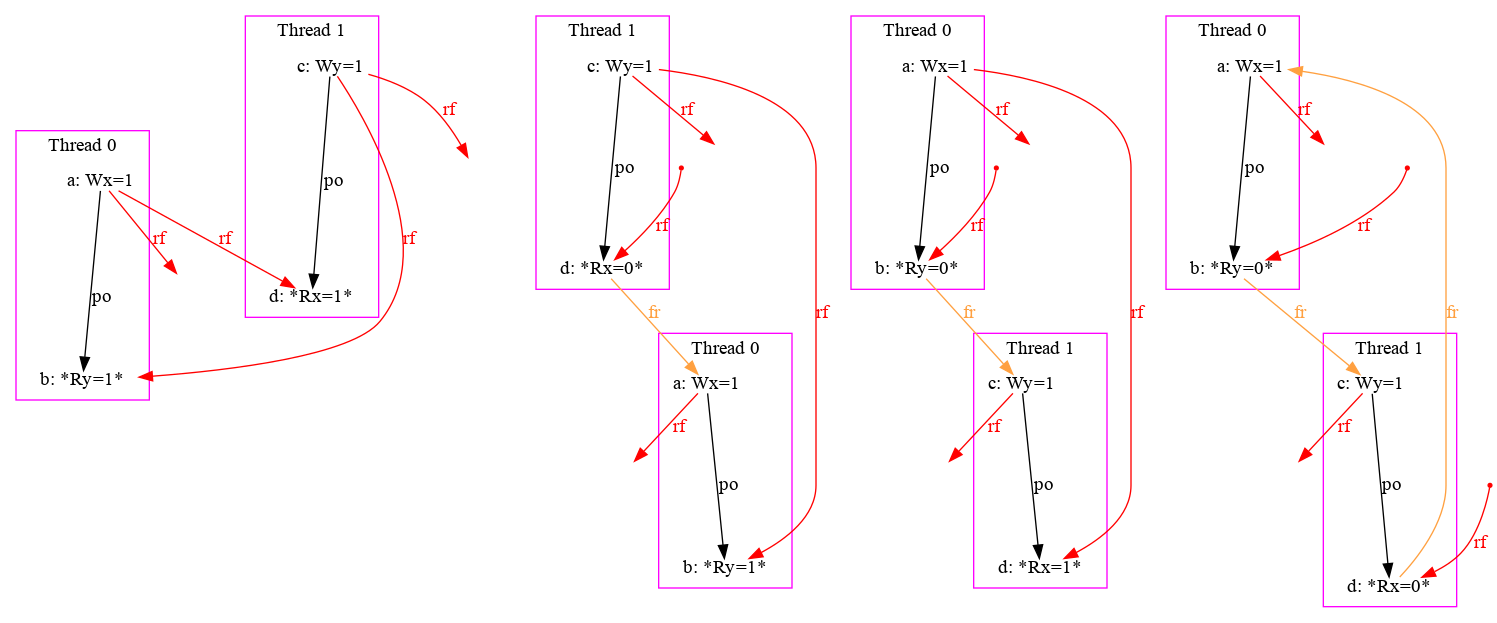
\includegraphics[width=\linewidth]{img/candidate.png}
\caption{The four candidate executions}
\end{figure}

\end{frame}



\begin{frame}{Verification of concurrent software}
\framesubtitle{A weak memory model: Operational semantics} %{Example: Store buffering (hardware)}
\begin{center}
\scalebox{0.7}{
\ttfamily
\begin{tabular}{ |>{\color{dkblue}}l | >{\color{dkred}}l| }
\hline
\multicolumn{2}{|l|}{ \{ x=0; y=0; \}} \tabularnewline \hline
P & Q \\ \hline
$p_0$ : $x \leftarrow 1$   & $q_0$: $y \leftarrow 1$   \\
$p_1$ : $r_p \leftarrow y$ & $q_1$: $r_q \leftarrow x$ \\
\hline
\end{tabular}
}
\end{center}

\begin{figure}
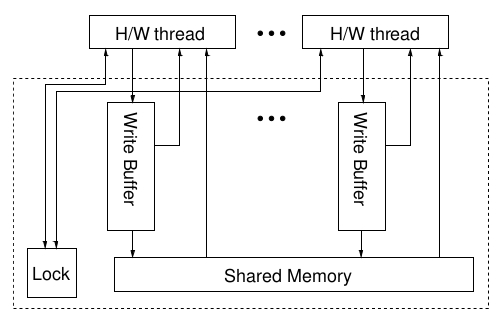
\includegraphics[scale=0.37]{img/x86-arch-full.png}
\caption{An x86-TSO abstract machine~\cite{sewell2010x86}}
%\label{fig:x86-arch}
\end{figure}
\end{frame}


%\framesubtitle{A weak memory model: Axiomatic semantics}

\begin{frame}{Verification of concurrent software}
\framesubtitle{A weak memory model: Axiomatic semantics}

\begin{itemize}
  \item 
\end{itemize}

\end{frame}





%\subsection{Актуальность}


\subsection{Problem statement (Цель исследования)}


\subsection{Task specification (Задачи исследования)}

1) 
2)
3)






















% Section and subsections will appear in the presentation overview
% and table of contents.
\section{First Main Section}

\subsection{First Subsection}

\begin{frame}{First Slide Title}{Optional Subtitle}
  \begin{itemize}
  \item {
    My first point.
  }
  \item {
    My second point.
  }
  \end{itemize}
\end{frame}

\subsection{Second Subsection}

% You can reveal the parts of a slide one at a time
% with the \pause command:
\begin{frame}{Second Slide Title}
  \begin{itemize}
  \item {
    First item.
    \pause % The slide will pause after showing the first item
  }
  \item {   
    Second item.
  }
  % You can also specify when the content should appear
  % by using <n->:
  \item<3-> {
    Third item.
  }
  \item<4-> {
    Fourth item.
  }
  % or you can use the \uncover command to reveal general
  % content (not just \items):
  \item<5-> {
    Fifth item. \uncover<6->{Extra text in the fifth item.}
  }
  \end{itemize}
\end{frame}

\section{Second Main Section}

\subsection{Another Subsection}

\begin{frame}{Blocks}
\begin{block}{Block Title}
You can also highlight sections of your presentation in a block, with it's own title
\end{block}
\begin{theorem}
There are separate environments for theorems, examples, definitions and proofs.
\end{theorem}
\begin{example}
Here is an example of an example block.
\end{example}
\end{frame}

% Placing a * after \section means it will not show in the
% outline or table of contents.
\section*{Summary}

\begin{frame}{Summary}
  \begin{itemize}
  \item
    The \alert{first main message} of your talk in one or two lines.
  \item
    The \alert{second main message} of your talk in one or two lines.
  \item
    Perhaps a \alert{third message}, but not more than that.
  \end{itemize}
  
  \begin{itemize}
  \item
    Outlook
    \begin{itemize}
    \item
      Something you haven't solved.
    \item
      Something else you haven't solved.
    \end{itemize}
  \end{itemize}
\end{frame}



% All of the following is optional and typically not needed. 
\appendix
\section<presentation>*{\appendixname}
\subsection<presentation>*{For Further Reading}

\begin{frame}[allowframebreaks]
  \frametitle<presentation>{Bibliography}
  \printbibliography
\end{frame}

\end{document}


